\section{Discussion} 
\label{sec:discussion}

\subsection{Planning Year 3 with Years 4--$N$ in mind}
\label{sec:gtr_1yr_horizon}

% Contextualize importance of thinking beyond just 1 yr Extended Mission
\tesss orbit is stable, in principle, for more than 1000 years~\citep{gangestad_high_2013}.
While minor mechanical failures should be expected on the timescale of a few 
years, it is plausible that the spacecraft could be operable for up to a decade.
Therefore, when choosing any particular plan for a one-year Extended Mission, it makes
sense to also consider the implications of an even longer Extended Mission.

% Preliminary discussion of immediate extensibility
A simple point is that \nhemi, \npole, and \shemiAvoid\:can all be inverted to their southern or northern complements for a fourth year of observing.
This will yield a comparable number of new planets to what they find in year 3 ($\mathcal{O}(1300)$ with $R_p<4R_\oplus$).
This would continue \tesss role as a planet-discovery machine, while also 
addressing the matter of refining ephemerides in order to enable detailed 
characterization with suitable instruments.

While our simulations show that observing opposite hemispheres in Years 3 and 4 
leads to many planet detections, we have not compared this strategy with 
observing the same hemisphere in both years (\textit{e.g.,} performing 
\nhemi\:in both Years 3 and 4). The latter approach might improve planet 
detection statistics, in particular with small and long-period planets.
An argument against such a strategy would be that it postpones refining 
the \tess planet ephemerides until Year 5.
We leave the detailed comparison for future work. 

In terms of the other strategies, \elong, \eshort, and \hemis\:are less 
obviously extensible to multiple years.
The main reasons to return to the ecliptic after performing \elong\:or 
\eshort\:would be to make \tesss survey truly `all-sky', and to perform \ktwo 
follow-up observations (see discussion below).
Of course, this would need to happen during intervals in which the Moon and 
Earth were not in the way.
\shemiAvoid\ would also achieve this goal.
%Continuous observations have serious value. 

%Leave the detailed characterization for \jwst, Spitzer, HST, ground-based 
%ELTs, and posterity.


% Move on to very-long term comments.
Any of our proposed scenarios could simply be repeated indefinitely,
as could possible two-year Extended Missions in which our scenarios 
would be followed by their respective complement hemispheres.
However, qualitatively novel trade-offs may arise when comparing two-year
Extended Missions.
For instance, after completing the Primary Mission, compare the 2-year
extension scenarios of \#1) two years of \hemis\ vs. \#2) repeating the 
Primary Mission for two years.
If we repeat the Primary Mission over 2 years, the northern
and southern CVZs get 1 additional year each of continuous observation.  
If we execute \hemis\:for 2 years, the northern and southern `long viewing
zones' each get 2 years of 14-day windowed observations. 
While each CVZ star receives the same total observing time, CVZ stars in \#1 
have a 1-year baseline, continuously sampled, while those in \#2 have a 2-year 
baseline, half-sampled.
Thus \#2 allows 2-transit detections of $P\lesssim1$ year planets over
$2\%$ of the sky.  \#1 allows 2-transit detections of
$P\lesssim6$ month planets over $1\%$ of the sky.  
In the competition between better time-sampling and longer baselines,
it is not clear which strategy is superior.

Another longer-term question is ``when will \tess hit the point of
diminishing returns?''  The `low-hanging fruit' of small planets
transiting bright stars at short orbital periods will become 
``picked over'' if \tess observes the same sky indefinitely.  
The most important
qualitative point of this memo, made in Fig.~\ref{fig:snrf_histogram},
is that after \tesss Primary Mission there will be many objects
remaining for which merely doubling the number of observed transits
will enable their detection.  Eventually though, once \tess is complete
for $R_p<4R_\oplus$ planets orbiting bright stars on $P<20\,\mathrm{day}$ 
orbits, more observations will
only allow us to probe out to longer orbital periods and dimmer stars.
We have not yet quantified when \tess will reach this
regime.

\subsection{The Ephemeris Problem}
\label{sec:ephemeris_times}

\paragraph{Analytic motivation}

For follow-up observations, we will often need to predict future times
of transits or occultations, ideally with an accuracy of an hour or
less. After enough time has passed that the uncertainty has grown to an
operationally significant value, we say that the ephemeris
has gone ``stale,'' \textit{i.e.,} it presents a major obstacle to many 
follow-up programs. For \tesss ground-based follow-up campaign, following up a 
planet
with a stale ephemeris would require much more observing time
for a successful result.  Likewise, for planning
space-based observations, for which observing time is always scarce,
it is extremely important to have a reliable and precise ephemeris.
For mass determination through the Doppler method, a stale transit
ephemeris adds uncertainty to the planetary mass measurements, by
increasing the number of effectively free parameters.

Consider then the problem of estimating $\sigma_{t_c}(T_x)$, the
uncertainty of the mid-transit time $\sigma_{t_c}$ for a given planet
at some time $T_x$ following its last-observed transit.  We begin
analytically: assume that the planet has $N_\mathrm{tra}=2$ observed
transits, spaced an orbital period $P=14$ days apart. Because that
period is one half the nominal \tess dwell time of a given pointing,
it represents the shortest period for which typically
$N_\mathrm{tra}=2$, and as such is the worst-case scenario for predicting
the times of future transits, amongst cases with $N_\mathrm{tra}>1$.
Given two mid-transit times, each measured with the time's uncertainty
$\sigma_0$, separated by $P$, the uncertainty of a future mid-transit
time can be derived by standard least-squares fitting and propagation
of errors (\textit{e.g.}~\citet{lyons_practical_1991}, Equation 2.18):

\begin{equation}
	\sigma_{t_c}(T_x) = \sigma_0 \sqrt{1 + 2 T_x / P + 2 (T_x / P)^2 }
\end{equation}
Note that for observing future transits, $E \equiv T_x / P$ is a positive 
integer, and the above equation can be re-expressed:
\begin{equation}
	\sigma_{t_c}(E) = \sigma_0 \sqrt{1 + 2 E + 2 E^2 },
\end{equation}
which is bounded by the simpler approximation: 
\begin{equation}
	\sigma_{t_c}(E) \lesssim \sigma_0 \left(1+\sqrt{2} E\right), 
\end{equation}
which is exact at $E=0$, has a maximum 8\% fractional error at $E=1$, and becomes increasingly accurate as $E$ increases. By $E=20$, the fractional error of the latter approximation is less than 1\%.

At 2-minute cadence, a typical value for the per-transit timing uncertainty is 
$\sigma_0 = 4$ minutes.
For example, if $T_x = 2$ years and $P = 2$ weeks, then $E \approx 50$, so 
$\sigma_{t_c}\approx 75\sigma_0$.
Hence the predicted $1\sigma$ uncertainty on its mid-transit time 
is 5 hours (two years later) or 10 hours (four years later).
 
 This leads to a simple rule of thumb: 
\begin{quotation}
  For a two-transit super-Earth, the $1\sigma$ uncertainty in the predicted 
  transit time, in hours, is numerically equal to about
  2$Y$, where $Y$ is the number of years after the Primary Mission.
\end{quotation}
If the transits are observed only at 30-minute cadence, then uncertainty will be roughly 4 times greater: $\sigma_0 \sim 16$ minutes. 
This claim (``$4\times$ greater'') is based on Figure 9 of~\citep{price_transit_2014}, a plot of the effects of finite cadence on timing precision. % note that they're using kepler data here 
We compared the precisions of 2-min and 30-min cadences for their specific example of $P=10$ days and a dwell time of 1 month.

On the other hand, Fig.~\ref{fig:Ntra_hist_primary} shows that 7 in 8 of the 
planets detected by \tesss Primary Mission will have $N_\mathrm{tra}>3$ and so 
their ephemerides should be better than the worst case example derived 
analytically above.
Rather than generalize the analytic equations, we resort to numerical simulations in order to predict the uncertainties of mid-transit times for planets expected to be discovered by \tesss Primary Mission.

\paragraph{Numerical analysis}
We start with the analytic form~\citet{price_transit_2014} derive for the per-transit uncertainty on the mid-transit time $\sigma_0$:
\begin{equation}
\sigma_{0} = \frac{1}{Q} \sqrt{ \frac{\tau T}{2} } \left( 1 - \frac{t}{3\tau} 
\right)^{-1/2}
	\label{eq:price_rogers_0}
\end{equation}
when $\tau\geq t$ and 
\begin{equation}
	\sigma_{0} = \frac{1}{Q} \sqrt{\frac{t T }{2}} \left( 1 - \frac{\tau}{3t} \right)^{-1/2}
	\label{eq:price_rogers}
\end{equation}
when $t > \tau$,
where $Q$ is the SNR per transit, $t$ is the cadence, $T$ is the transit duration, and $\tau$ is the ingress (or egress) time.
We have all the latter terms from our yield simulation, and show the resulting 
distribution of $\sigma_0$ in Fig.~\ref{fig:uncertainty_tc_hist}.
Indeed, our suggested $\sigma_0$ of about 4 minutes for postage stamps and 16 
minutes for full frame images is reasonable, which is good because we computed 
the former from the $t\rightarrow0$ limit of Eq.~\ref{eq:price_rogers_0} 
originally derived by~\citet{carter_analytic_2008}.
\begin{figure}[!t]
	\centering
	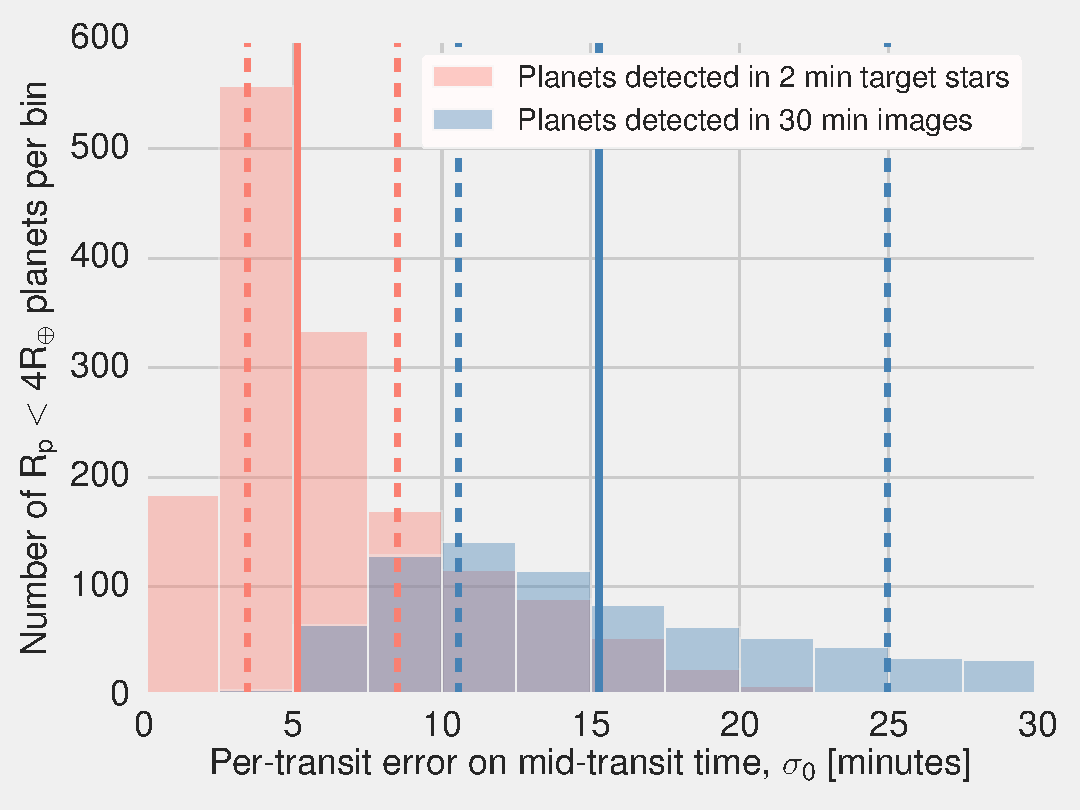
\includegraphics[scale=1.]{figures/mid_transit_time_vs_cadence.pdf}
	\caption{Uncertainty of mid-transit time on a single transit, $\sigma_{t_c}$, for all detected $R_p<4R_\oplus$ planets from the Primary Mission as computed from Eq.~\protect\ref{eq:price_rogers}.
		Solid lines are medians, dashed lines are 25$^\mathrm{th}$ and 75$^\mathrm{th}$ percentiles.
	}
	\label{fig:uncertainty_tc_hist}
\end{figure}
\begin{figure}[!t]
	\centering
	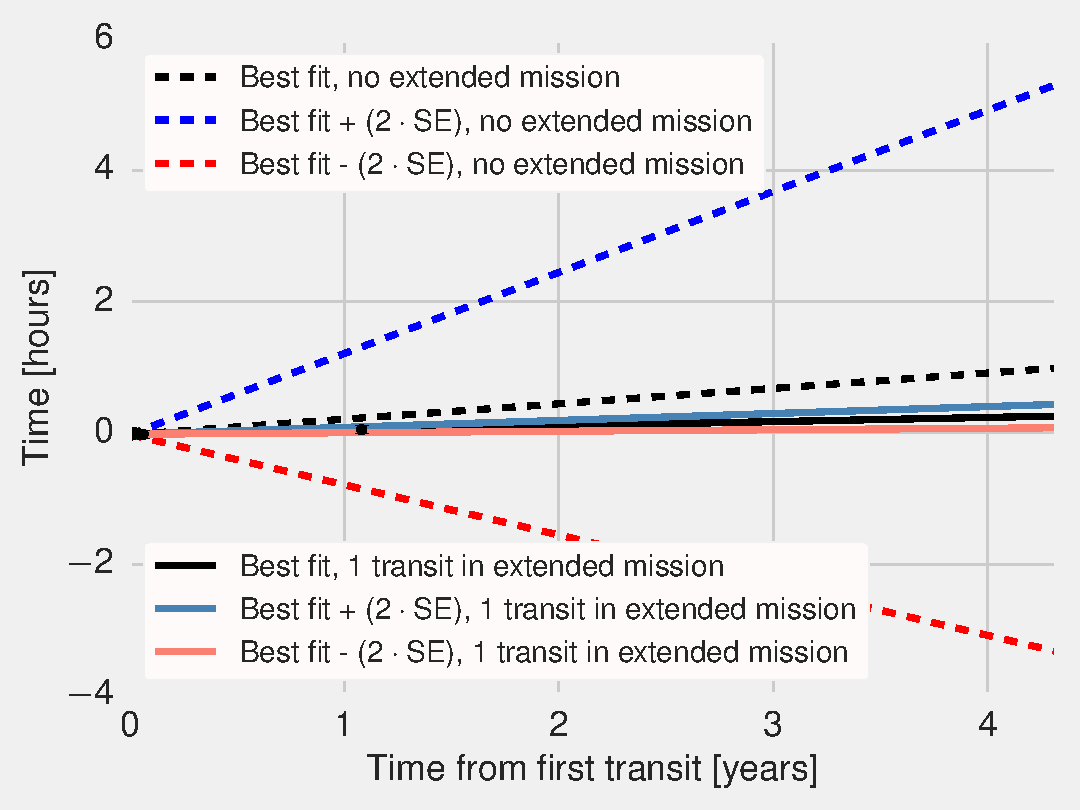
\includegraphics[scale=1.]{figures/lowering_uncertainty_on_midtransit_via_extra_point.pdf}
	\caption{	Observed mid-transit times (dots) and best fits to a linear ephemeris (lines).
		The dashed lines fit 4 data points from a nominal planet.
		The solid lines do the same, but with an additional transit observed one year
		later.
		`SE' is the standard error on the slope which multiplied by 1.96 (rounded to 2 in the legend) gives a 95\% confidence interval between the blue and orange lines.
	}
	\label{fig:lowering_uncertainty_tc}
\end{figure}

Given the distributions on per-transit uncertainty of $t_c$, we then took an example planet with 4 transits.
We drew ``observed'' mid-transit times from a Gaussian with zero mean and standard deviation $\sigma_{0}$, and then ran a linear least squares regression. 
We then added just one data point 1 year after the final observed transit, and repeated the regression.
This produces a cartoon-plot, Fig.~\ref{fig:lowering_uncertainty_tc}, which confirms two expected points:
\begin{enumerate}
	\item Years after the initial discovery, the uncertainty of mid-transit time is of order hours.
	\item If we detect an additional transit 1 year after the final observed transit from the Primary Mission, the uncertainty on the mid-transit time decreases by an order of magnitude.
\end{enumerate}

\begin{figure*}[!t]
	\centering
	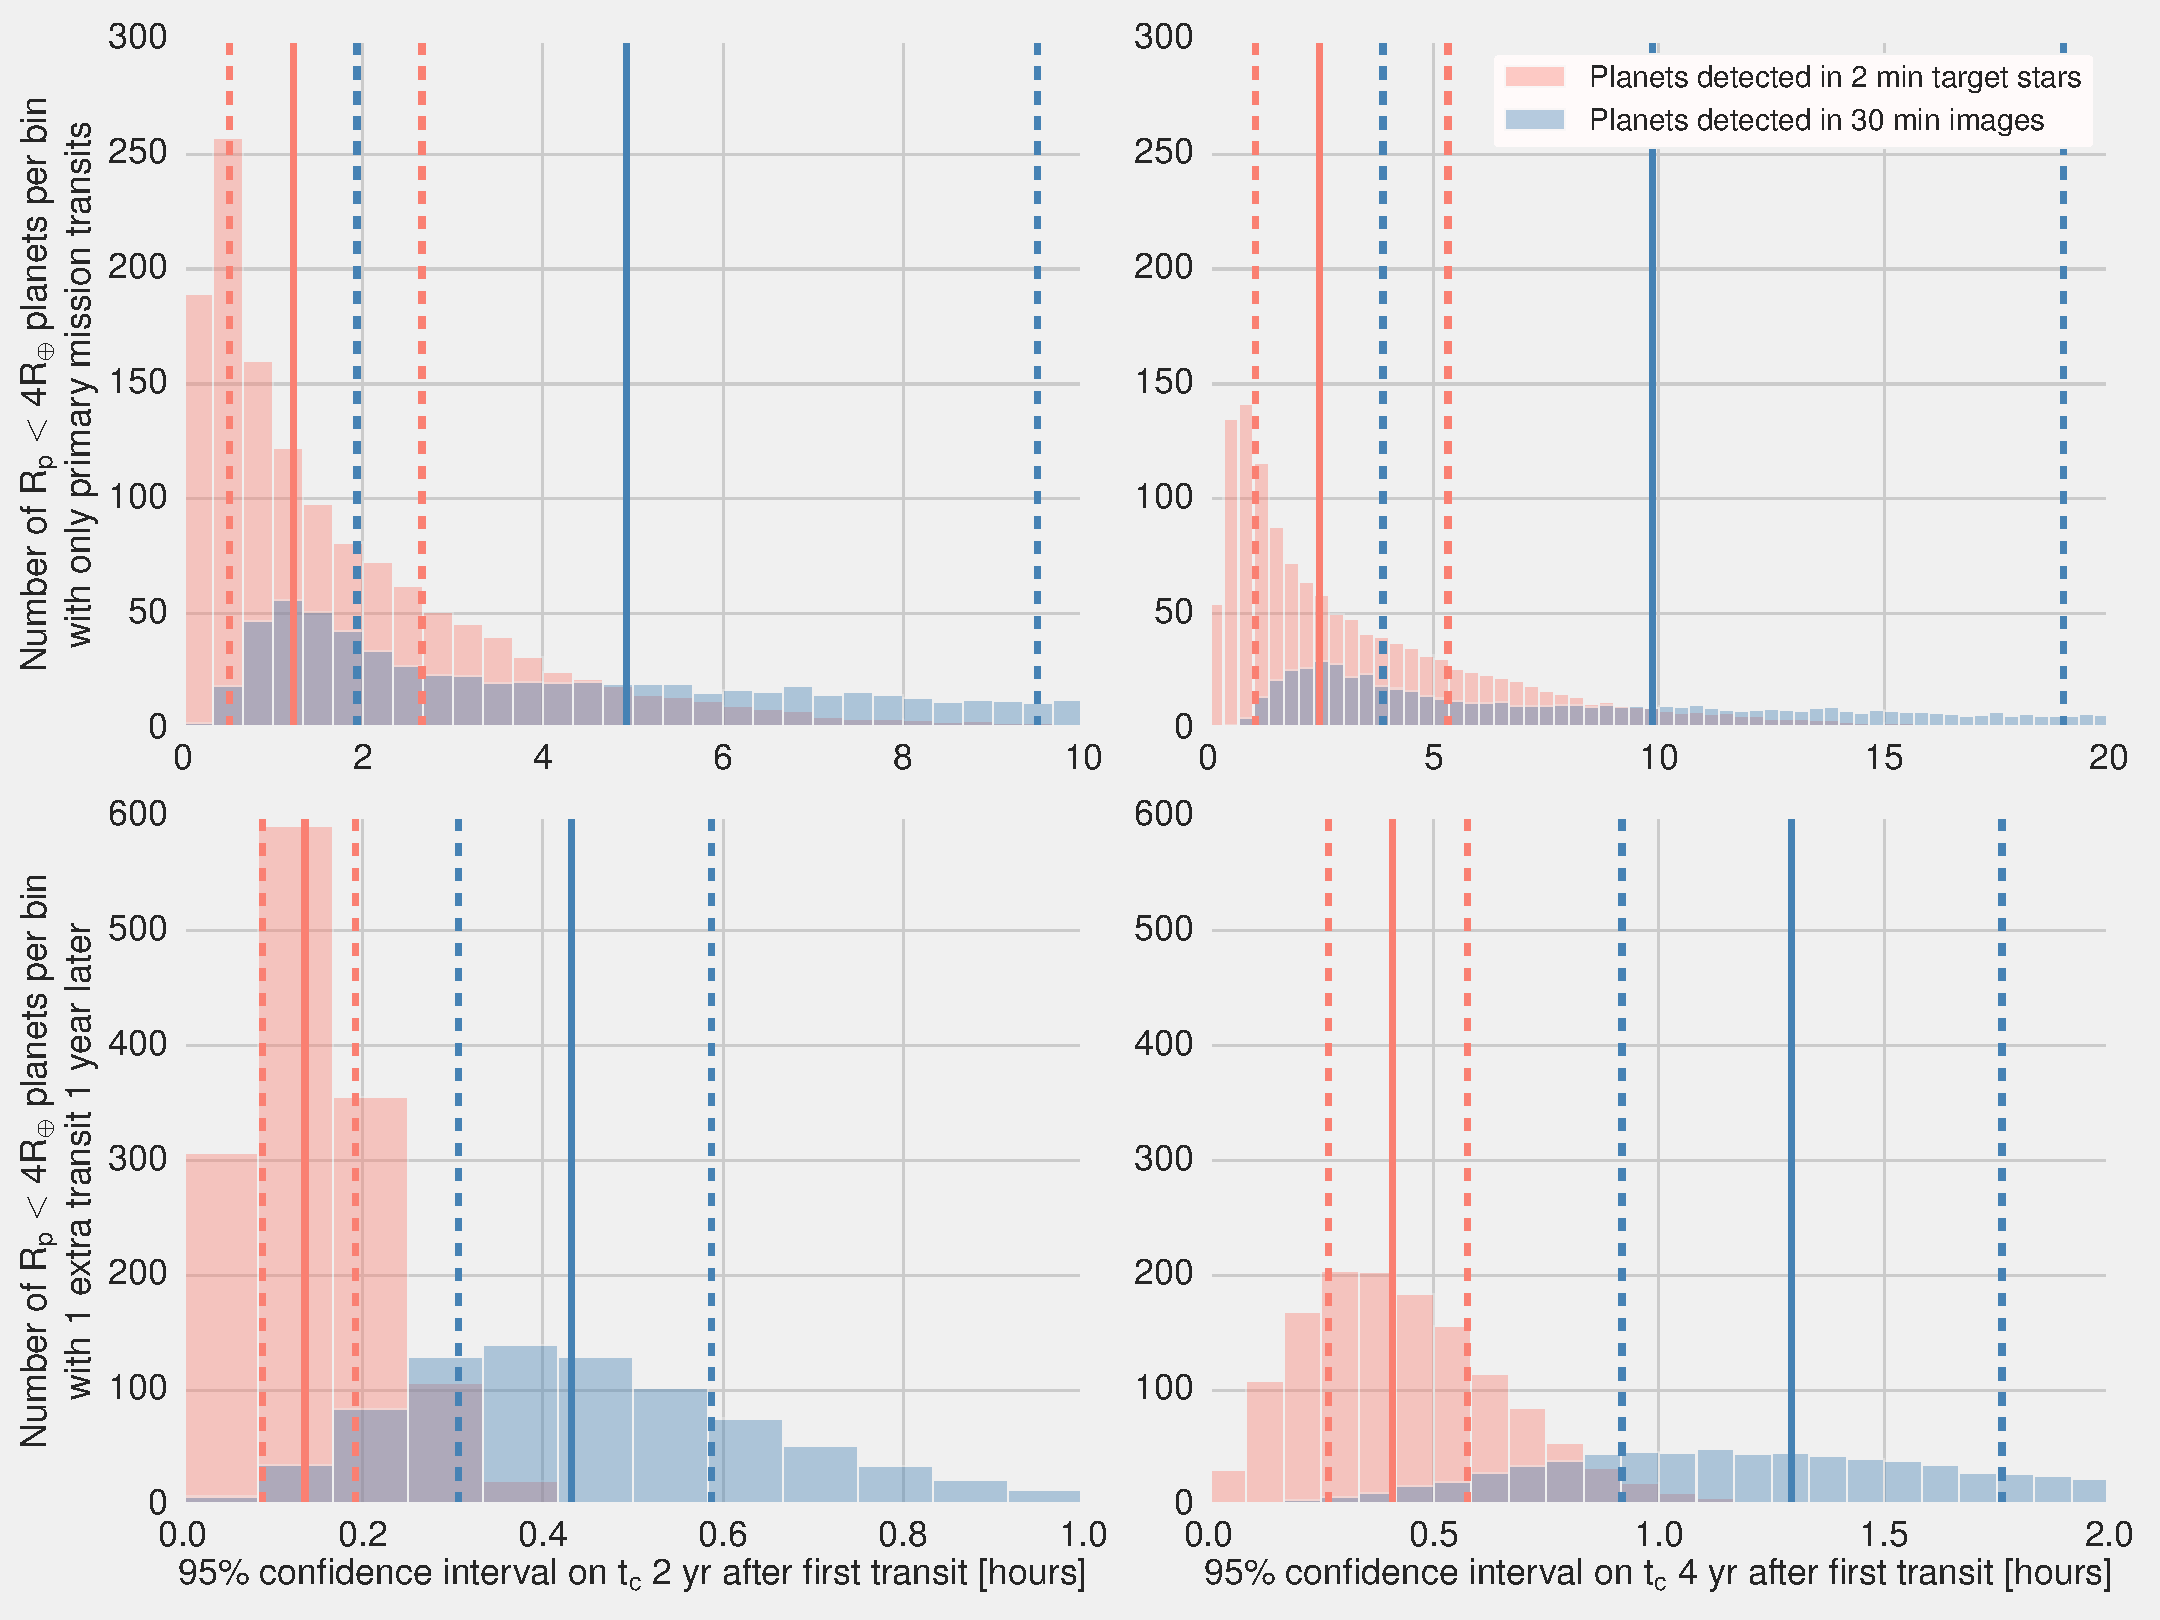
\includegraphics[scale=1.]{figures/confidence_interval_gets_better.pdf}
	\caption{\textit{Top row}: histogram of 95\% confidence intervals 2 (\textit{left}) and 4 (\textit{right}) years following the first detected transit in the Primary Mission.
		20 minute bins.
		\textit{Bottom row}: histogram of 95\% confidence intervals 2 (\textit{left}) and 4 (\textit{right}) years following the first detected transit in the Primary Mission, but with an additional data point added to the analog of Fig.~\protect\ref{fig:lowering_uncertainty_tc} one year after the transit in the initial time series (5 minute bins).
		Note that the top row's timescale is an order of magnitude greater than the bottom row.
		Solid lines are medians, dashed lines are 25$^\mathrm{th}$ and 75$^\mathrm{th}$ percentiles.
	} %all in ephemeris_uncertainties.ipynb
	\label{fig:conf_interval_gets_better}
\end{figure*}
We proceed by repeating the above procedure for every planet, and evaluate typical 95\% confidence intervals (``uncertainties'', loosely) for $t_c$, at typical times after the first transits, for all of our detected planets.
Specifically, we take them at $T_x=2$ and $4$ years, and get Fig.~\ref{fig:conf_interval_gets_better}.
This figure confirms (top left panel) our analytic expectation that the uncertainty of mid-transit times in hours should be somewhat less than twice the number of years after \tess first observes the planet at 2-min cadence, since most such planets have $N_\mathrm{tra}\geq4$.
It also confirms our rough expectation that the uncertainty on FFI mid-transit 
times is roughly 4 times that of postage stamps, although the uncertainties on 
FFIs have a much broader tail than PSs.

More importantly, Fig.~\ref{fig:conf_interval_gets_better} emphasizes the importance of refining \tesss ephemerides: if we do not, the typical \tess planet will have many hours of uncertainty on its mid-transit time a few years following its detection.
If we do follow-up with an Extended Mission, we will be able to predict when 
the planet transits to $\lesssim1$ hour for many more years.
This argues strongly for an Extended Mission which, whether over 1 or 2 years, re-observes many if not all of the targets that \tess detects in its Primary Mission. 
The smallest-radius Earths and super-Earths may otherwise be much more 
difficult to follow up.


\subsection{Risks and Caveats}
\label{sec:risks_caveats}
\paragraph{Risk that planet detection simulation gets yield wrong:}
What is the risk that we over or under-estimated \tesss planet yield, either in the Primary Mission, or in any given Extended Mission?
We summarized the assumptions that went into our yield calculations in Sec.~\ref{sec:input_assumptions}.
We made them believing that they were all good enough for useful relative comparisons of different sky-scanning scenarios,
even if they are not correct in absolute terms to better than $\approx$50\%.

Highlighting a few of these assumptions, in order of what we feel is decreasing
concern:
\begin{itemize}
\item [1.) We assume no knowledge of the outcomes of prior transit searches.]
  	As indicated in the text, this assumption is worst for the
        \elong\:and \eshort\:scenarios, for which \ktwo and \tesss
        overlap will be important.  Estimating the magnitude of our
        error, assume \ktwo will have observed $70\%$ of the sky in
        the $|\beta|<6^\circ$ band about the ecliptic by 2019.  Of the
        1169 `new' $R_p<4R_\oplus$ planets that \tess detects in
        \elong, 239 of them are within $|\beta|<6^\circ$ of the
        ecliptic, and thus roughly 167 will already have been observed by
        \ktwo (assuming the same stars were selected in \ktwo 
        observations).  
        This simple estimate quantifies our global error in reporting `new'
        planets near the ecliptic ($\sim 15\%$ will not be truly `new'), but 
        neglects the issue of merging the
        two datasets to discover long period planets.  This latter
        opportunity could be an important reason to actually do
        \elong\:or \eshort\:and thus demands detailed study, which we
        recommend below.
	    
	\item [2.) We use a SNR threshold of 7.3.] This number was computed by~\citetalias{Sullivan_2015} based on the argument that it would be a sufficient threshold to give one statistical false positive per $2\times10^5$ light curves.
	Applying the same criterion to full frame images would lead to more than one false positive, since full frame images come from a much larger sample of stars.
	Any pipeline that is written to work with \tess data will confront this problem:
	processing $10^8$ vs. $10^6$ stars requires different false positive thresholds.
	Extrapolating from~\citetalias{Sullivan_2015}'s Fig 15, a threshold sufficient to give 0.05 false positives per $2\times10^5$ light curves, or 1 false positive per $4\times10^6$ light curves (as from our full frame images), is roughly 7.5.
	Making the same ad-hoc estimate that~\citetalias{Sullivan_2015} did and multiplying by 1.03 for the expected drop in SNR from cosmic ray noise gives a SNR threshold of 7.7 for full frame images.
	Considering our Fig.~\ref{fig:snrf_histogram} (and noting the black line is for the sum of postage stamp and full frame image detections), adopting a SNR threshold of 7.7 for FFIs would mean a loss of $\sim30\times4=120$ planets over two years, or 60 of what we claim are `detected planets' from full frame images in 1 year's Extended Mission.	 We also note that our model lacks any accounting for time-correlated noise and the probabilistic nature of the signal recovery process, which are likely to be more important factors than the purely white-noise statistical fluctuations.
	
	
	\item [3.) We use synthetic stars from a single galactic model (TRILEGAL).]
	One check on the robustness of this model would be to compare with other galactic models like GALAXIA~\citep{sharma_galaxia_2011} or the Besa\c con model~\citep{robin2003synthetic}.
	The simplest analytic model, applicable given that \tesss limiting distance for $R_p<4R_\oplus$ detections is $\lesssim 1\ \mathrm{kpc}$, is a distribution of stars uniform in the radial direction and with an exponential profile in the vertical direction. 
	Independent of our numerical simulation,~\citet{winn_searchable_2013} used such a galactic profile, with occurrence rates inferred from \kepler Q1-6. Our results are in order-of-magnitude agreement, with ours being slightly higher, likely due to our incorporation of~\citet{dressing_occurrence_2015}'s M dwarf occurrence rates.
	
	It might eventually be best to use the real star catalog that \tesss Target Selection Working Group is assembling. However, until \gaia DR2 (Q4 2017), this will likely come with large uncertainties on stellar radii, given the difficulty of distinguishing giants and sub-giants from M dwarfs without proper motions.
	An additional challenge is in companion fractions.
	
	While we recommend that these broader checks be performed in future \tess yield calculations, they are excessive for the purposes of this report given that we only used the nearest, brightest, stars ($d\lesssim\mathrm{1kpc}, I_c\lesssim16$), with a simple prescription for background contamination, in evaluating \tesss $R_p<4R_\oplus$ detections.
	The uncertainties become much greater if we try to estimate detections of giant planets and false positives throughout the galactic disk.
	That said, we take~\citetalias{Sullivan_2015}'s cross-checks (cf Fig. 5 of that paper) against actual surveys of the local stellar population as indicative that we probably have the number of nearby stars, as well as their properties, correct for the accuracy required in this work.
	%!WINN! #3, 4, 5, 7 not specific to Extended Missions, right?
	%!BOUMA! right. But they should still be here?
	
	\item [4.) At least 2 transits for detection:] recall Figs.~\ref{fig:Ntra_hist} and~\ref{fig:Ntra_hist_primary}.
	If we were to use a more stringent criteria, for instance at least 3 transits for detection as the \kepler pipeline currently does, we would lose $\mathcal{O}(200)$ of the planets detected in the Primary Mission, and $\mathcal{O}(100)$ from the Extended Missions.
	This assumption disproportionately affects long-period planets.
	
%	\item[6.) Multiple planet system distributions:] we assumed that we could approximate the occurrence rates for transiting multiple planet systems as repeated draws from the single-planet occurrence distributions (with independent probability) with added impositions of co-planarity and orbital stability.
	
	
	\item [5.) We neglect instrument aging, spacecraft systematics, etc.]
	To our knowledge detailed models do not currently exist for how \tesss 
	optics and CCDs will degrade with time.
%	\todo[inline]{talk with Goddard people about this}
	We are also assuming that, as with \ktwo\!, time-correlated spacecraft level systematics can be removed in post-processing.
	These assumptions are reasonable at our current state of pre-flight knowledge, and will need to be changed accordingly as the mission progresses.
	If we were to assume a gradual decline in photometric performance, for instance from an increased number of dead or `hot' pixels, the relative Extended-Mission-to-Extended-Mission comparisons would remain identical.
	The absolute Extended-Mission-to-primary-Mission yields would decrease.
	
	\item [6.) We do not consider the efficacy of processing pipeline.]
	For instance, \hemis\:will come with period ambiguities and aliasing problems imposed by its 14 day sampling at the `continuous' viewing zones.
	Similar issues are generic across Extended Missions for which we detect a small number of transits in the Primary Mission, and then a small number of transits in the Extended Mission.
	
	A robust way to approach this problem would be to generate a synthetic simulated \tess dataset, \textit{i.e.}, at the image-level, rather than at the idealized phase-folded SNR level from this work, for each Extended Mission's observations.
	Then actually perform astrometry on injected stars, extract light curves, de-trend them, and find their transits.
	This exercise would likely also be a useful way to prepare the SPOC and broader community for what we expect the era of \tess photometry to entail in terms of data quality.	
\end{itemize}

